%!TEX root = ../dissertation.tex
\begin{savequote}[75mm]
	At the root of all politics is the universal language of conflict.
	\qauthor{Schattschneider}
\end{savequote}


\chapter{Introduzione}
\label{chap:introduzione}

\section{Il contesto storico}
A partire dalle elezioni americane del 2008, la politica ha capito di dover fare i conti con i social media per rendere le proprie campagne elettorali realmente efficaci. In quell'anno Barack Obama puntò molto sul suo sito internet my.barackobama.com, sul suo profilo    Myspace e sul suo profilo Facebook. All'epoca, il ventiquattrenne Chris Hughes, co-fondatore di quest'ultimo social network, era anche direttore della parte online della campagna del futuro presidente.

Da allora, negli ultimi 12 anni, tutte le campagne elettorali si sono progressivamente spo-state online e sui social media.
Simbolo ne sono le elezioni del 2016 in cui l'azienda Cambridge Analytica diretta da Steve Bennon ha condotto una profilazione di massa di profili Facebook (indebitamente collezionati) utilizzando una versione semplificata dei Big5.

Questa operazione che ha unito \textit{behavioral science}, \textit{data analytics} con il \textit{micro-targeted advertisements}, ha avuto esiti sicuramente positivi, anche se difficilmente quantificabili \citep{rathi2019}, per la vittoria di Trump. In quelle elezioni infatti hanno fatto la differenza una manciata di voti in alcuni stati chiave.

Più in generale, l'utilizzo di questo tipo di campagne basate sull'utilizzo di informazioni personali, sulla cui raccolta si fondano i social network, è diventata una pratica comune nel marketing e non stupisce che sia utilizzata anche per trasmettere contenuti politici. Questo fenomeno segue il costante aumento di persone connesse in rete in tutto il mondo. Proprio nel 2020 il numero di persone che utilizzano i social media è arrivato a 3.96 miliardi, pari  al 51\% della popolazione globale \citep{kemp2020} [Fig. \ref{fig:usoSocial}], con un aumento di 160 miliardi rispetto ai dati di inizio febbraio \citep{kemp2}. Il numero di persone che comunica tramite social è in rapido aumento, solo quest'anno è cresciuto del 10\% (376 milioni in più rispetto al 2019), e il trend non accenna a diminuire. In media le persone spendono circa due ore e mezza al giorno sui social e nel 40\% dei casi lo fanno per lavoro,  dimostrando quanto questi strumenti stiano diventando parte fondamentale delle nostre vite per diverse ragioni, non solo ricreative [Fig. \ref{fig:usosocial2}].
L'utilizzo delle piattaforme commerciali sembra essere diventato ancora più predominante durante la recente pandemia, come dimostra uno studio \citep{gwi2020} secondo cui in Italia è cresciuto addirittura del 43\% (in linea con l'aumento globale medio).
\begin{figure}
	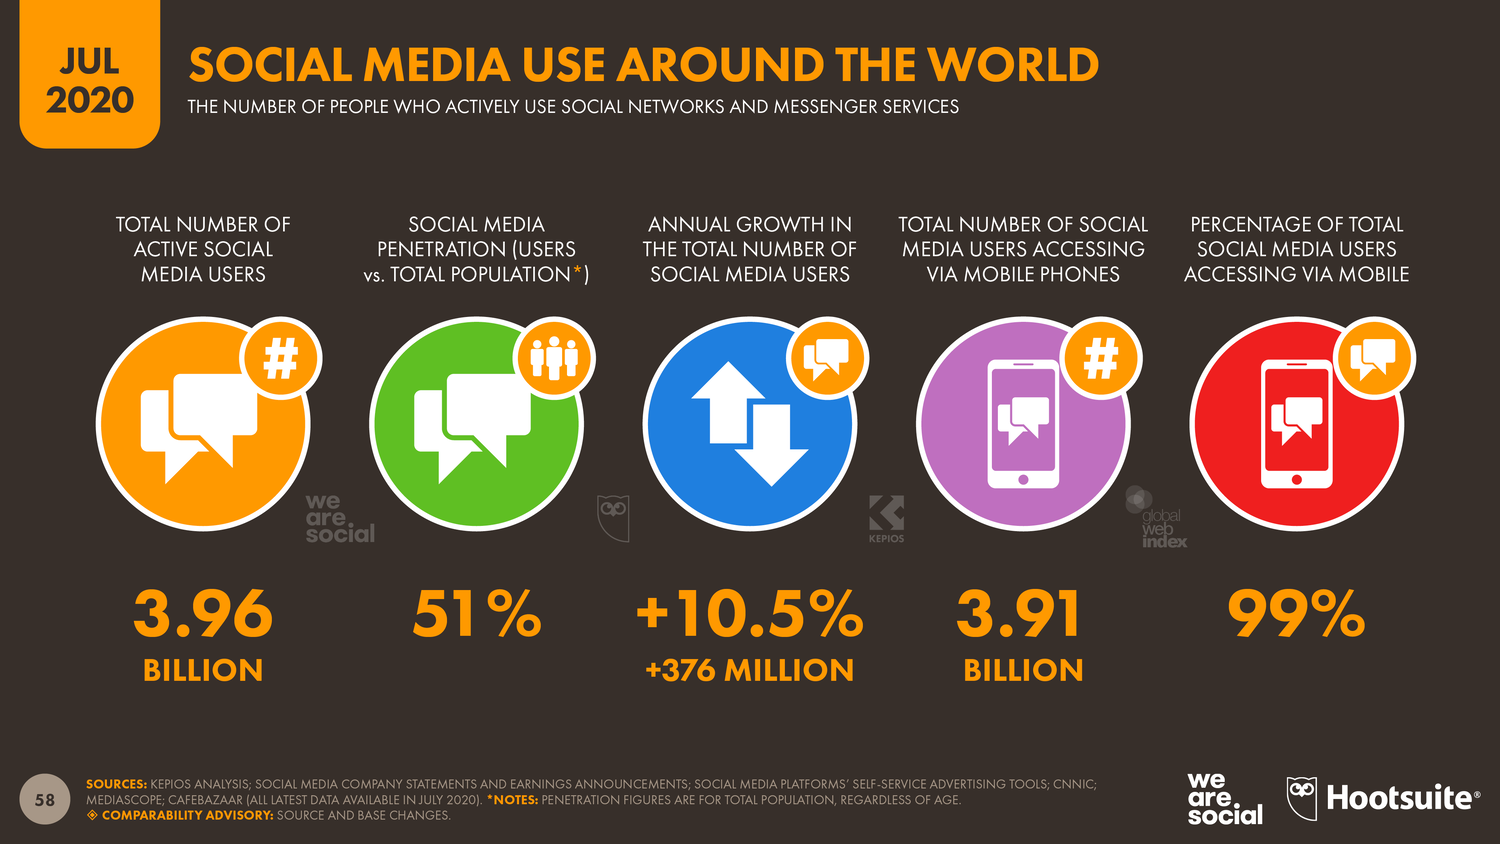
\includegraphics[width=\textwidth]{figures/social_media}
	\caption{L'utilizzo dei social media aggiornato a giugno 2020. Immagine pubblicata all'interno del "Digital 2020: july global statshot"}
	\label{fig:usoSocial}
\end{figure}


Più di 2 miliardi e 600 milioni di persone usano almeno una volta al mese Facebook, che si conferma la piattaforma più utilizzata al mondo, ma l'utilizzo di un social non ne esclude altri. Twitter, che conta "solo" 326 milioni di utenti attivi al mese, riscontra una sovrapposizione dei suoi utenti con quelli di Facebook dell'88\% dei casi, il che mostra  come diverse piattaforme, con diverse regole e stili comunicativi, si completino a vicenda svolgendo ruoli  diversi e complementari. Ad esempio, benchè Twitter sia uno dei social con meno utenti attivi al mese (si colloca al sedicesimo posto), risulta essere il quinto sito più visitato sul totale del traffico globale a causa del suo utilizzo da parte dei politici per la trasmissione di comunicati stampa seguiti da persone anche non attive sulla piattaforma. La comunicazione politica viene affidata spesso a questo social di microblogging, come emerge anche dal Digital News Report 2020 \citep{newman2020} dell'università di Oxford, in cui il social dei cinguettii risulta essere una fonte di notizie di attualità per l'11\% dei soggetti, percentuale che sommata al 46\% di intervistati che invece utilizzano Facebook per cercare news ed informarsi, rende evidente l'importanza di questi nuovi canali di comunicazione.
\begin{figure}
	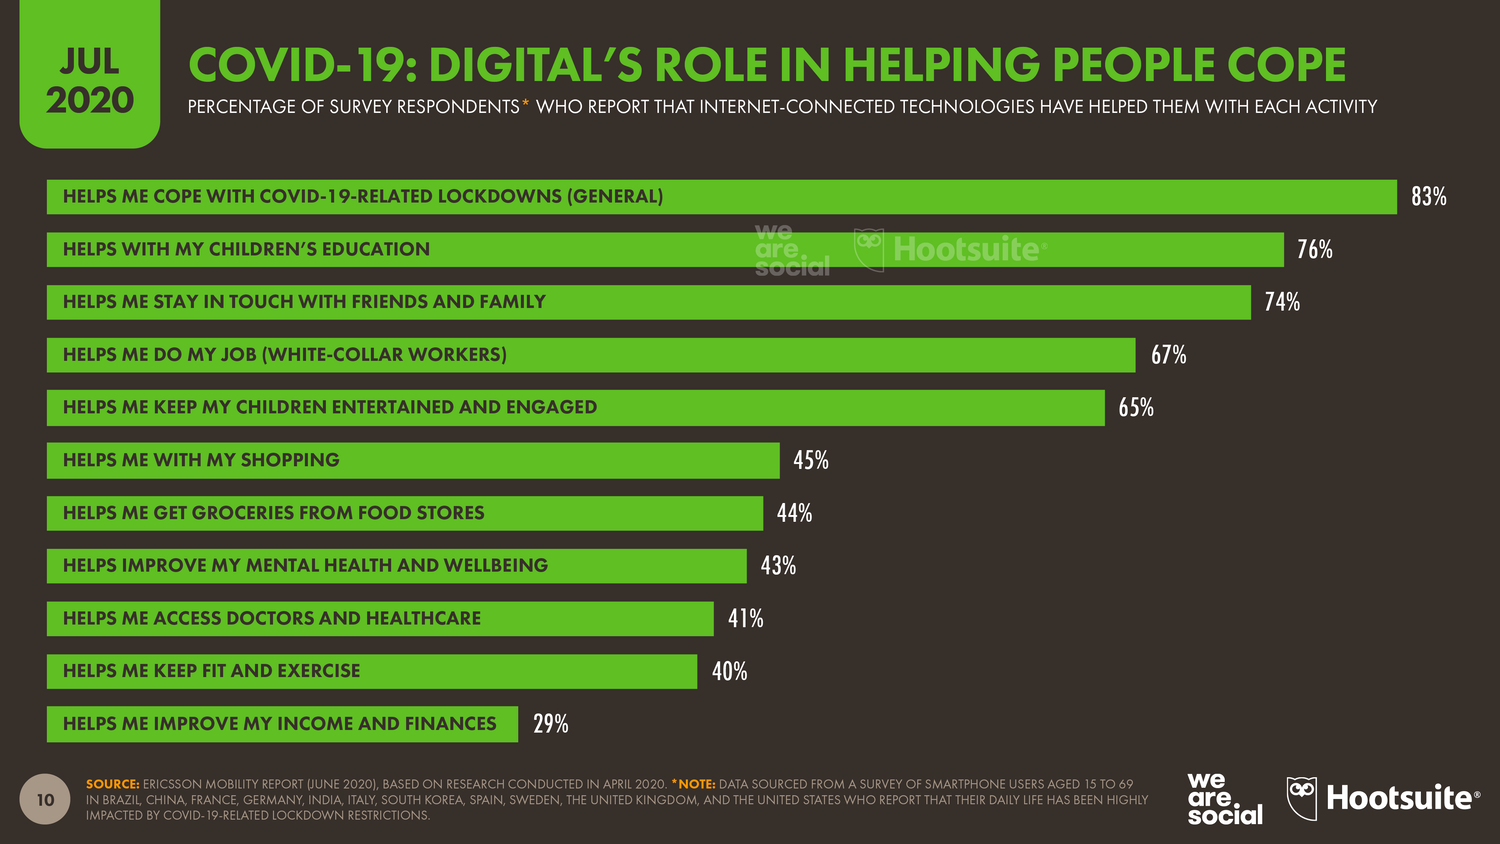
\includegraphics[width=\textwidth]{figures/usosocial2}
	\caption{I settori della vita in cui internet è stato più utile durante la pandemia. Immagine pubblicata all'interno del "Digital 2020: july global statshot"}
	\label{fig:usosocial2}
\end{figure}

Se da una parte i social network hanno visto un enorme sviluppo in questi anni, andando a definire aspetti importanti della vita come la comunicazione politica e l'informazione gio-rnaliera di una fetta sempre maggiore della popolazione, dall'altra hanno generato alcuni fenomeni negativi come la diffusione di disinformazione e la crescita dei discorsi d'odio che in alcuni casi sfociano addirittura in veri e propri \textit{hate crime} \citep{chan2015}.
Un esempio diventato tristemente celebre è quello del \textit{Pizza Gate}. Sempre durante la campagna elettorale americana del 2016, alcune email sottratte a John Podesta, responsabile della campagna elettorale di Hillary Clinton, vengono pubblicate da WikiLeaks. A partire da questo materiale, alcuni account Twitter di politici conservatori e  personaggi dell'\textit{alt-right} iniziano a diffondere teorie del complotto riguardanti presunti abusi su minori e riti satanici condotti da esponenti democratici in alcuni ristoranti di Washington. Le tragiche conseguenze di questa vicenda ci mostrano come "Fake News Brought Real Guns" \citep{Kang2016}. Infatti, a seguito della campagna di disinformazione online, si è generata una campagna di odio online sulle pagine delle pizzerie coinvolte che ha portato poi Edgar M. Welch, un giovane ventottenne della Carolina del Nord, a fare fuoco (offline) all'interno di una delle pizzerie al centro del falso scandalo (fortunatamente senza ferire nessun*).

Nel corso degli ultimi anni la società civile, le grandi corporazioni che comprano spazi pubblicitari sui social media e i social media stessi hanno discusso di come contrastare l'odio online, prendendo contromisure che vanno dalla rimozione di account particolarmente problematici, alla categorizzazione automatizzata (o semi-automatizzata) dei contenuti problematici, fino alla modifica dei termini del servizio che regolano le discussioni all'interno delle varie piattaforme.
Già nel 2017, un articolo pubblicato sul Wall Street Journal \citep{nicas2017} segnava l'avvio della prima "Adpocalypse", termine che letteralmente significa “apocalisse delle pubblicità” e indica il  boicottaggio massiccio da parte di grandi aziende delle piattaforme social, con l'obiettivo di far cambiare le regole alla base dell' organizzazione dei contenuti.  Nel primo caso, a seguito della pubblicazione di alcuni \textit{screenshots} sul Twitter del giornalista Jack Nicas, in cui pubblicità di grandi aziende come Coca-Cola venivano suggerite su Youtube in relazione a video inneggianti al razzismo se non addirittura a messaggi di propaganda di terroristi islamici vicini all'Isis, molte importanti aziende decisero di bloccare le sponsorizzazioni fino a quanto Google non fosse stata in grado di evitare questo tipo di eventi moderando meglio l'odio sulle sue piattaforme.  Da allora diverse volte episodi di lobbismo contro i social media hanno puntato alla revisione delle regole di \textit{content curation}. L'ultimo attacco in ordine temporale è avvenuto nel giugno 2020, quando l'azienda di telecomunicazioni Verizon ha iniziato a ritirare le sue pubblicità da Facebook \citep{Kari2020}, riprendendo un appello della campagna "Stop hate for profit" \citep{stophate2020}. La questione si è in qualche modo risolta tramite un accordo interno alla Global Alliance for Responsible Media (GARM), di cui fa parte anche lo stesso Facebook, in cui si individuano delle linee guida per definire in modo comune l'\textit{hate speech} e per aumentare la sicurezza digitale \citep{wfa2019}.


Un altro evento recente di estrema rilevanza riguarda l'account Twitter di Donald Trump. Lo scorso 29 Maggio, per la prima volta, il social network di microblogging ha moderato un contenuto proprio del presidente degli Stati Uniti \citep{tacopino2020}.  In seguito alla dichiarazione del \textit{Tycoon} riguardo le proteste scoppiate dopo l'uccisione di Jorge Floyd, in cui afferma che “Quando cominciano i saccheggi, si inizia a sparare”, il media statunitense ha deciso di sovrapporre al tweet una “public interest notice” in quanto l'affermazione sarebbe una “glorification of violence” non in linea con gli standard della comunità [Fig. ~\ref{trump}]. Benchè l'affermazione non sia stata rimossa dalla piattaforma per la sua rilevanza pubblica, questo episodio rappresenta un punto cruciale nell'evoluzione della propaganda politica, e della sua relazione con l'odio, nel contesto online.

\begin{wrapfigure}{r}{7cm}
	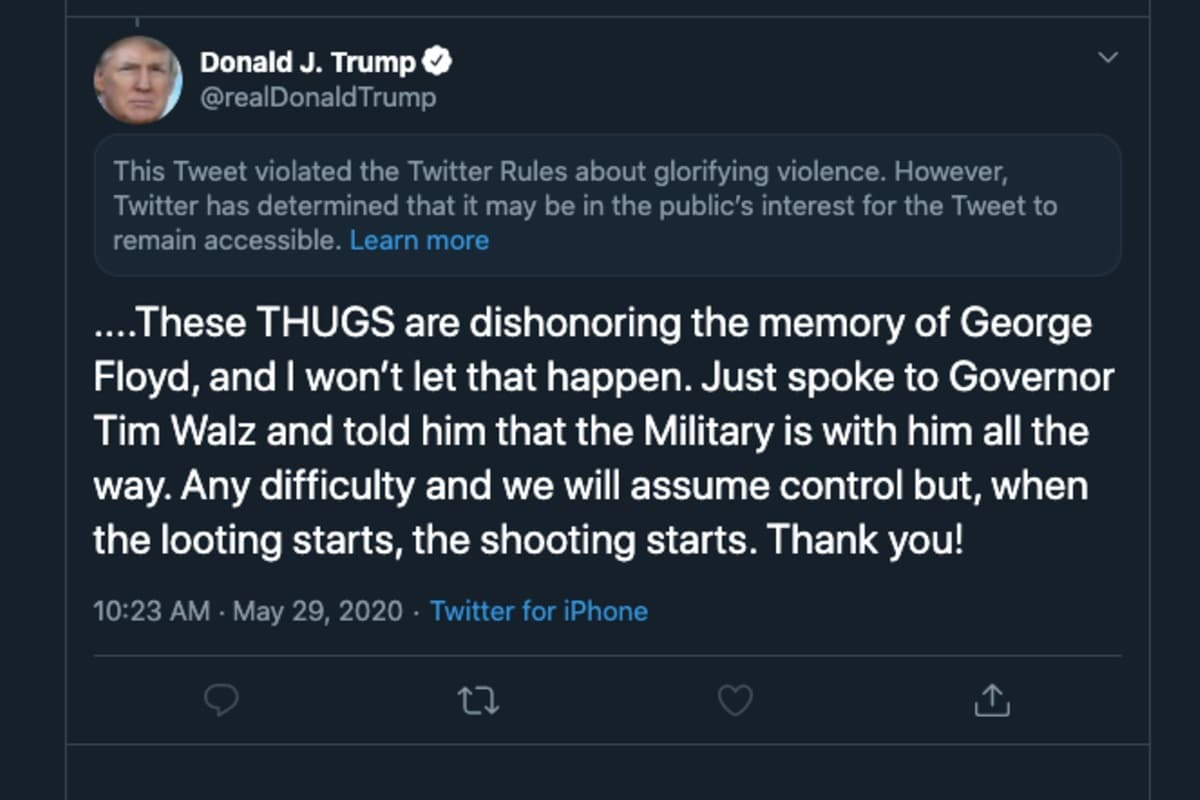
\includegraphics[width=\linewidth]{figures/trump}
	\caption{Il post di Trump contestato da Twitter.}
	\label{trump}
\end{wrapfigure}

Se da una parte le multinazionali si ritrovano a dover fare pressioni sui social network affinchè limitino l'odio, le stesse piattaforme diventano moderatrici addirittura della massima carica politica statunitense, proprio per prevenire ulteriori episodi di violenza, dimostrando come queste piattaforme si trovino al centro, nel bene e nel male, del dibattito contemporaneo sulla libertà di parola.

%Le considerazioni fin qui riportate, determinano l’importanza di una indagine scientifica sull’odio online.
%Le campagne politiche online sono state sempre più frequenti negli ultimi 12 anni, questo anche in relazione al progressivo aumento globale dell'utilizzo dei social media in diversi aspetti della vita quotidiana. Contemporaneamente sono emerse diverse problematiche relative all'odio su queste piattaforme e alla loro relazione  con episodi di violenza offline, soprattutto nel contesto del dibattito politico, aumentando la necessità di una moderazione da parte dei social stessi, fino ad arrivare alla moderazione di uno dei politici più influenti del mondo,  

A partire da tali considerazioni sulla relazione tra odio online e politica, in questa tesi si indaga la relazione tra il \textit{negative campaign} e l' \textit{hate speech}. L'obiettivo della ricerca è comprendere come alcuni tipi di campagna politica possano generare violenza online. Il nostro auspicio è che i risultati raggiunti possano fornire  strumenti scientifici utili alla creazione di strategie efficaci per la riduzione dei livelli di odio online, anche cominciando con il far comprendere ai politici gli effetti della loro comunicazione.
% https://journals.sagepub.com/doi/abs/10.1177/1354068815601787  -->Contagious Euroscepticism: The impact of Eurosceptic support on mainstream party positions on European integration
%https://ejpr.onlinelibrary.wiley.com/doi/epdf/10.1111/j.1475-6765.1980.tb00737.x ---> NINE SECOND‐ORDER NATIONAL ELECTIONS – A CONCEPTUAL FRAMEWORK FOR THE ANALYSIS OF EUROPEAN ELECTION RESULTS

\section{I contenuti della tesi}
Il presente lavoro si apre con una rassegna bibliografica della teoria del \textit{negative campaign} (capitolo "\nameref{chap:negative}") e dell'\textit{hate speech online} (capitolo "\nameref{chap:hate}"). Dopo aver presentato l'origine della presente ricerca (“\nameref{chap:ricerca}”) si passa poi ad analizzare nel dettaglio il "Barometro dell'odio" sviluppato da Amnesty International durante la campagna elettorale per le elezioni europee in Italia del 2019, che fornisce il database di partenza per le ulteriori codifiche effettuate per il presente elaborato (capitolo "\nameref{chap:metodologia}"). Seguiranno le analisi svolte con i principali risultati (capitolo "\nameref{chap:risultati}") e le conclusioni con le riflessioni finali (capitolo "\nameref{chap:conclusioni}").





